% generated by Plantuml 1.2022.7       
\definecolor{plantucolor0000}{RGB}{241,241,241}
\definecolor{plantucolor0001}{RGB}{24,24,24}
\definecolor{plantucolor0002}{RGB}{173,209,178}
\definecolor{plantucolor0003}{RGB}{0,0,0}
\definecolor{plantucolor0004}{RGB}{200,41,48}
\definecolor{plantucolor0005}{RGB}{132,190,132}
\definecolor{plantucolor0006}{RGB}{3,128,72}
\definecolor{plantucolor0007}{RGB}{169,220,223}
\definecolor{plantucolor0008}{RGB}{179,141,34}
\definecolor{plantucolor0009}{RGB}{255,255,68}
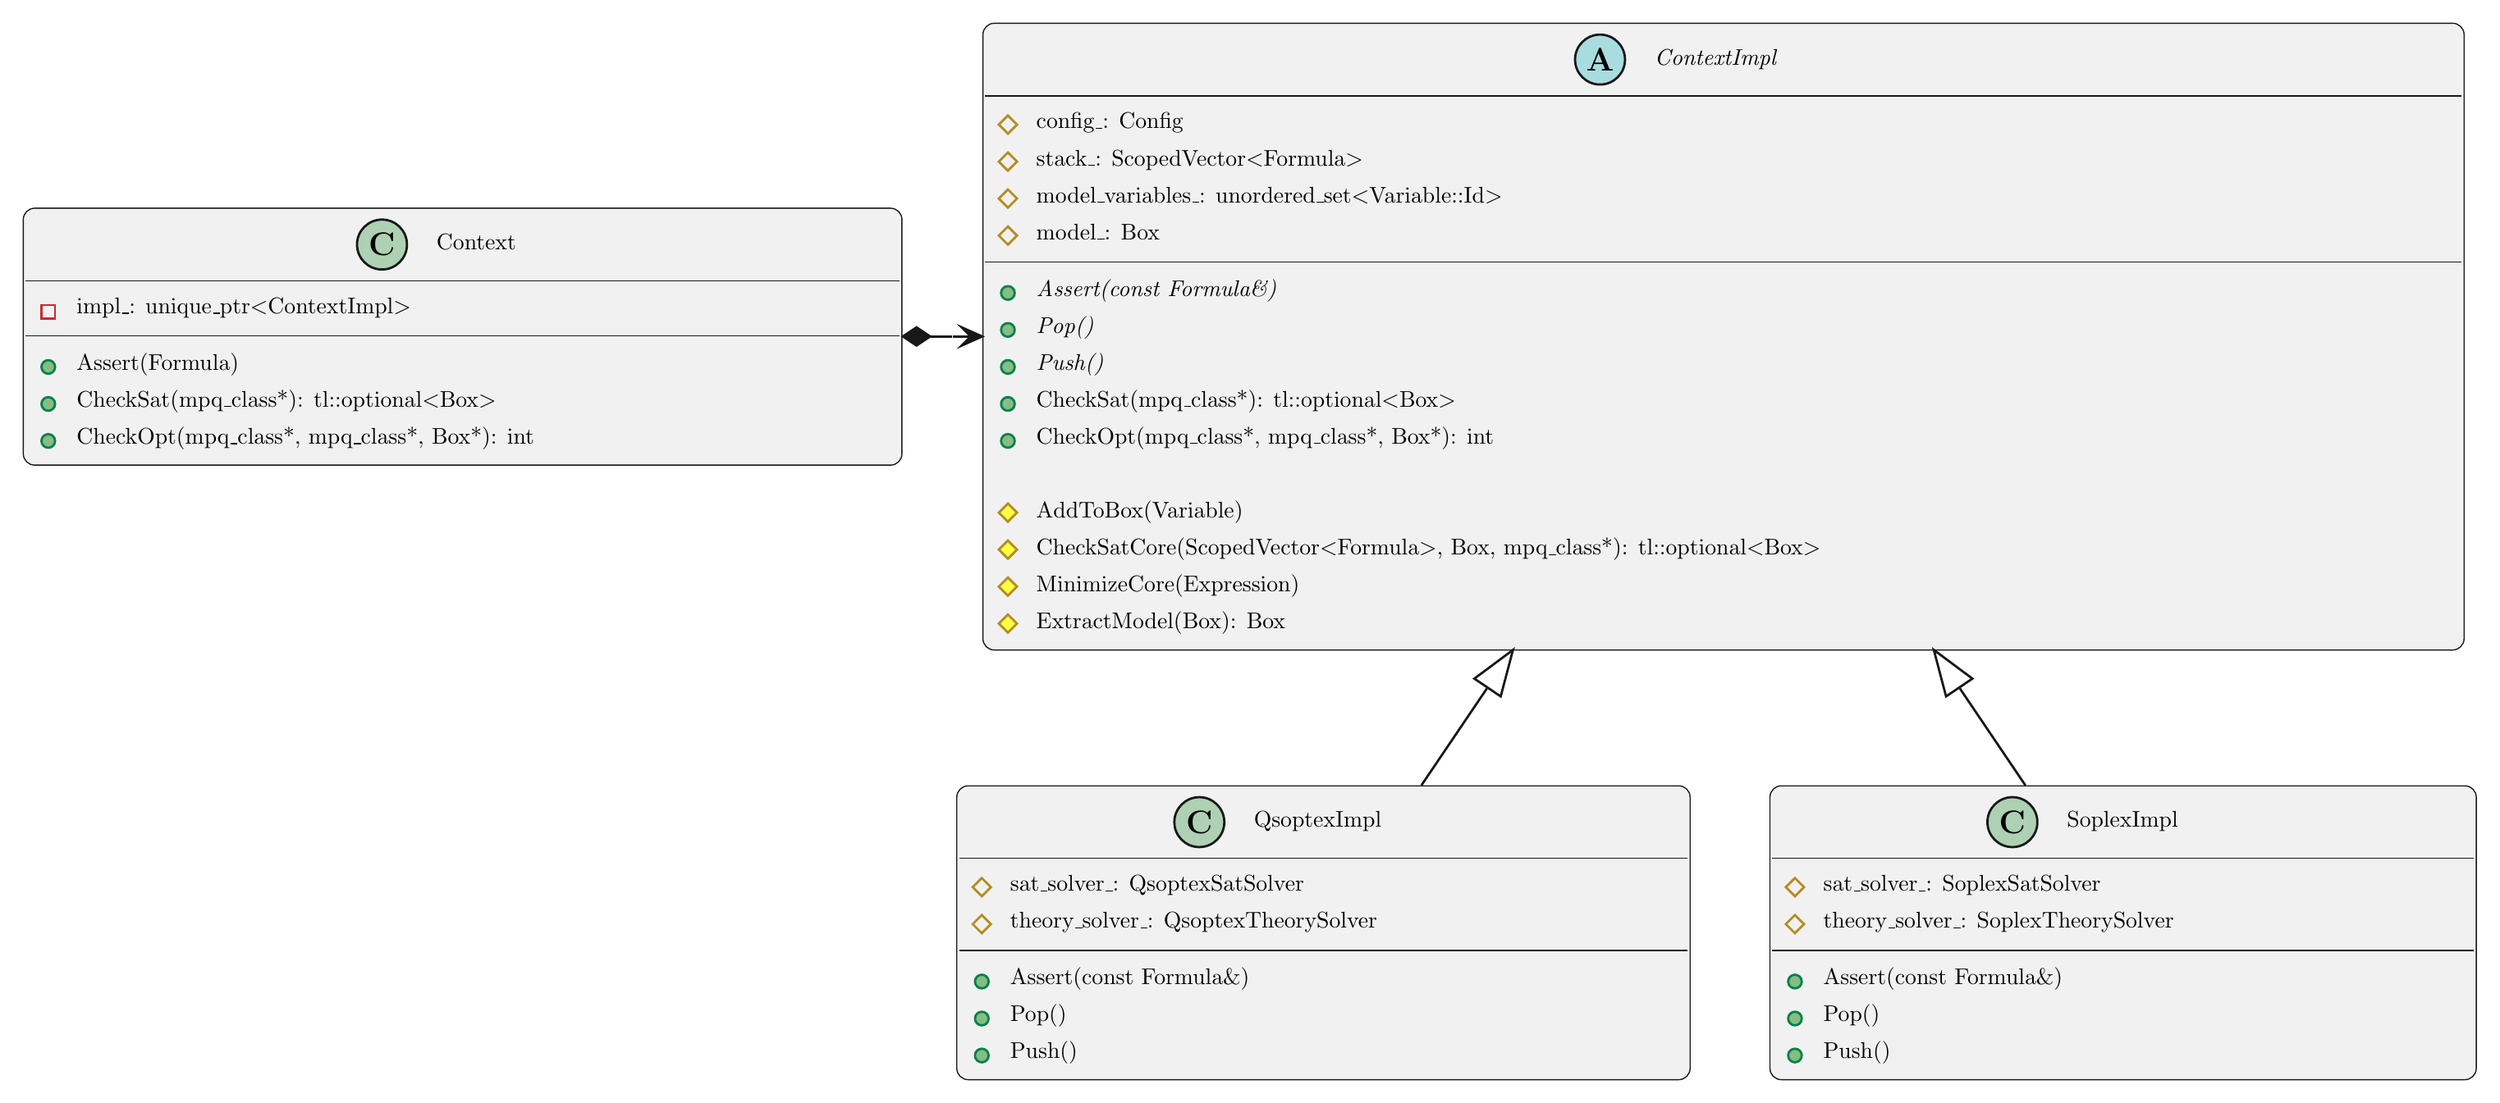
\begin{tikzpicture}[yscale=-1
,pstyle0/.style={color=plantucolor0001,fill=plantucolor0000,line width=0.5pt}
,pstyle1/.style={color=plantucolor0001,fill=plantucolor0002,line width=1.0pt}
,pstyle2/.style={color=plantucolor0001,line width=0.5pt}
,pstyle4/.style={color=plantucolor0006,fill=plantucolor0005,line width=1.0pt}
,pstyle6/.style={color=plantucolor0008,line width=1.0pt}
,pstyle7/.style={color=plantucolor0008,fill=plantucolor0009,line width=1.0pt}
,pstyle8/.style={color=plantucolor0001,line width=1.0pt}
,pstyle9/.style={color=plantucolor0001,fill=plantucolor0001,line width=1.0pt}
]
\draw[pstyle0] (7pt,93.5pt) arc (180:270:5pt) -- (12pt,88.5pt) -- (388.8453pt,88.5pt) arc (270:360:5pt) -- (393.8453pt,93.5pt) -- (393.8453pt,196.6875pt) arc (0:90:5pt) -- (388.8453pt,201.6875pt) -- (12pt,201.6875pt) arc (90:180:5pt) -- (7pt,196.6875pt) -- cycle;
\draw[pstyle1] (164.9298pt,104.5pt) ellipse (11pt and 11pt);
\node at (164.9298pt,104.5pt)[]{\textbf{\Large C}};
\node at (185.4298pt,96.3516pt)[below right,color=black]{Context};
\draw[pstyle2] (8pt,120.5pt) -- (392.8453pt,120.5pt);
\draw[color=plantucolor0004,line width=1.0pt] (15pt,131.1484pt) rectangle (21pt,137.1484pt);
\node at (27pt,124.5pt)[below right,color=black]{impl\_: unique\_ptr\textless ContextImpl\textgreater };
\draw[pstyle2] (8pt,144.7969pt) -- (392.8453pt,144.7969pt);
\draw[pstyle4] (18pt,158.4453pt) ellipse (3pt and 3pt);
\node at (27pt,148.7969pt)[below right,color=black]{Assert(Formula)};
\draw[pstyle4] (18pt,174.7422pt) ellipse (3pt and 3pt);
\node at (27pt,165.0938pt)[below right,color=black]{CheckSat(mpq\_class*): tl::optional\textless Box\textgreater };
\draw[pstyle4] (18pt,191.0391pt) ellipse (3pt and 3pt);
\node at (27pt,181.3906pt)[below right,color=black]{CheckOpt(mpq\_class*, mpq\_class*, Box*): int};
\draw[pstyle0] (429.5pt,12pt) arc (180:270:5pt) -- (434.5pt,7pt) -- (1076.5945pt,7pt) arc (270:360:5pt) -- (1081.5945pt,12pt) -- (1081.5945pt,278.1563pt) arc (0:90:5pt) -- (1076.5945pt,283.1563pt) -- (434.5pt,283.1563pt) arc (90:180:5pt) -- (429.5pt,278.1563pt) -- cycle;
\draw[color=plantucolor0001,fill=plantucolor0007,line width=1.0pt] (701.1892pt,23pt) ellipse (11pt and 11pt);
\node at (701.1892pt,23pt)[]{\textbf{\Large A}};
\node at (721.6892pt,14.8516pt)[below right,color=black]{\textit{ContextImpl}};
\draw[pstyle2] (430.5pt,39pt) -- (1080.5945pt,39pt);
\draw[pstyle6] (440.5pt,47.6484pt) -- (444.5pt,51.6484pt) -- (440.5pt,55.6484pt) -- (436.5pt,51.6484pt) -- cycle;
\node at (449.5pt,43pt)[below right,color=black]{config\_: Config};
\draw[pstyle6] (440.5pt,63.9453pt) -- (444.5pt,67.9453pt) -- (440.5pt,71.9453pt) -- (436.5pt,67.9453pt) -- cycle;
\node at (449.5pt,59.2969pt)[below right,color=black]{stack\_: ScopedVector\textless Formula\textgreater };
\draw[pstyle6] (440.5pt,80.2422pt) -- (444.5pt,84.2422pt) -- (440.5pt,88.2422pt) -- (436.5pt,84.2422pt) -- cycle;
\node at (449.5pt,75.5938pt)[below right,color=black]{model\_variables\_: unordered\_set\textless Variable::Id\textgreater };
\draw[pstyle6] (440.5pt,96.5391pt) -- (444.5pt,100.5391pt) -- (440.5pt,104.5391pt) -- (436.5pt,100.5391pt) -- cycle;
\node at (449.5pt,91.8906pt)[below right,color=black]{model\_: Box};
\draw[pstyle2] (430.5pt,112.1875pt) -- (1080.5945pt,112.1875pt);
\draw[pstyle4] (440.5pt,125.8359pt) ellipse (3pt and 3pt);
\node at (449.5pt,116.1875pt)[below right,color=black]{\textit{Assert(const Formula\&)}};
\draw[pstyle4] (440.5pt,142.1328pt) ellipse (3pt and 3pt);
\node at (449.5pt,132.4844pt)[below right,color=black]{\textit{Pop()}};
\draw[pstyle4] (440.5pt,158.4297pt) ellipse (3pt and 3pt);
\node at (449.5pt,148.7813pt)[below right,color=black]{\textit{Push()}};
\draw[pstyle4] (440.5pt,174.7266pt) ellipse (3pt and 3pt);
\node at (449.5pt,165.0781pt)[below right,color=black]{CheckSat(mpq\_class*): tl::optional\textless Box\textgreater };
\draw[pstyle4] (440.5pt,191.0234pt) ellipse (3pt and 3pt);
\node at (449.5pt,181.375pt)[below right,color=black]{CheckOpt(mpq\_class*, mpq\_class*, Box*): int};
\node at (449.5pt,197.6719pt)[below right,color=black]{ };
\draw[pstyle7] (440.5pt,218.6172pt) -- (444.5pt,222.6172pt) -- (440.5pt,226.6172pt) -- (436.5pt,222.6172pt) -- cycle;
\node at (449.5pt,213.9688pt)[below right,color=black]{AddToBox(Variable)};
\draw[pstyle7] (440.5pt,234.9141pt) -- (444.5pt,238.9141pt) -- (440.5pt,242.9141pt) -- (436.5pt,238.9141pt) -- cycle;
\node at (449.5pt,230.2656pt)[below right,color=black]{CheckSatCore(ScopedVector\textless Formula\textgreater , Box, mpq\_class*): tl::optional\textless Box\textgreater };
\draw[pstyle7] (440.5pt,251.2109pt) -- (444.5pt,255.2109pt) -- (440.5pt,259.2109pt) -- (436.5pt,255.2109pt) -- cycle;
\node at (449.5pt,246.5625pt)[below right,color=black]{MinimizeCore(Expression)};
\draw[pstyle7] (440.5pt,267.5078pt) -- (444.5pt,271.5078pt) -- (440.5pt,275.5078pt) -- (436.5pt,271.5078pt) -- cycle;
\node at (449.5pt,262.8594pt)[below right,color=black]{ExtractModel(Box): Box};
\draw[pstyle0] (418pt,348pt) arc (180:270:5pt) -- (423pt,343pt) -- (735.8427pt,343pt) arc (270:360:5pt) -- (740.8427pt,348pt) -- (740.8427pt,467.4844pt) arc (0:90:5pt) -- (735.8427pt,472.4844pt) -- (423pt,472.4844pt) arc (90:180:5pt) -- (418pt,467.4844pt) -- cycle;
\draw[pstyle1] (524.7714pt,359pt) ellipse (11pt and 11pt);
\node at (524.7714pt,359pt)[]{\textbf{\Large C}};
\node at (545.2714pt,350.8516pt)[below right,color=black]{QsoptexImpl};
\draw[pstyle2] (419pt,375pt) -- (739.8427pt,375pt);
\draw[pstyle6] (429pt,383.6484pt) -- (433pt,387.6484pt) -- (429pt,391.6484pt) -- (425pt,387.6484pt) -- cycle;
\node at (438pt,379pt)[below right,color=black]{sat\_solver\_: QsoptexSatSolver};
\draw[pstyle6] (429pt,399.9453pt) -- (433pt,403.9453pt) -- (429pt,407.9453pt) -- (425pt,403.9453pt) -- cycle;
\node at (438pt,395.2969pt)[below right,color=black]{theory\_solver\_: QsoptexTheorySolver};
\draw[pstyle2] (419pt,415.5938pt) -- (739.8427pt,415.5938pt);
\draw[pstyle4] (429pt,429.2422pt) ellipse (3pt and 3pt);
\node at (438pt,419.5938pt)[below right,color=black]{Assert(const Formula\&)};
\draw[pstyle4] (429pt,445.5391pt) ellipse (3pt and 3pt);
\node at (438pt,435.8906pt)[below right,color=black]{Pop()};
\draw[pstyle4] (429pt,461.8359pt) ellipse (3pt and 3pt);
\node at (438pt,452.1875pt)[below right,color=black]{Push()};
\draw[pstyle0] (776pt,348pt) arc (180:270:5pt) -- (781pt,343pt) -- (1081.96pt,343pt) arc (270:360:5pt) -- (1086.96pt,348pt) -- (1086.96pt,467.4844pt) arc (0:90:5pt) -- (1081.96pt,472.4844pt) -- (781pt,472.4844pt) arc (90:180:5pt) -- (776pt,467.4844pt) -- cycle;
\draw[pstyle1] (882.7377pt,359pt) ellipse (11pt and 11pt);
\node at (882.7377pt,359pt)[]{\textbf{\Large C}};
\node at (903.2377pt,350.8516pt)[below right,color=black]{SoplexImpl};
\draw[pstyle2] (777pt,375pt) -- (1085.96pt,375pt);
\draw[pstyle6] (787pt,383.6484pt) -- (791pt,387.6484pt) -- (787pt,391.6484pt) -- (783pt,387.6484pt) -- cycle;
\node at (796pt,379pt)[below right,color=black]{sat\_solver\_: SoplexSatSolver};
\draw[pstyle6] (787pt,399.9453pt) -- (791pt,403.9453pt) -- (787pt,407.9453pt) -- (783pt,403.9453pt) -- cycle;
\node at (796pt,395.2969pt)[below right,color=black]{theory\_solver\_: SoplexTheorySolver};
\draw[pstyle2] (777pt,415.5938pt) -- (1085.96pt,415.5938pt);
\draw[pstyle4] (787pt,429.2422pt) ellipse (3pt and 3pt);
\node at (796pt,419.5938pt)[below right,color=black]{Assert(const Formula\&)};
\draw[pstyle4] (787pt,445.5391pt) ellipse (3pt and 3pt);
\node at (796pt,435.8906pt)[below right,color=black]{Pop()};
\draw[pstyle4] (787pt,461.8359pt) ellipse (3pt and 3pt);
\node at (796pt,452.1875pt)[below right,color=black]{Push()};
\draw[pstyle8] (406.26pt,145pt) ..controls (406.26pt,145pt) and (413.04pt,145pt) .. (415.89pt,145pt);
\draw[pstyle9] (429.19pt,145pt) -- (420.19pt,141pt) -- (424.19pt,145pt) -- (420.19pt,149pt) -- (429.19pt,145pt) -- cycle;
\draw[pstyle8] (424.19pt,145pt) -- (416.19pt,145pt);
\draw[pstyle9] (394.26pt,145pt) -- (400.26pt,149pt) -- (406.26pt,145pt) -- (400.26pt,141pt) -- (394.26pt,145pt) -- cycle;
\draw[pstyle8] (651.38pt,300.11pt) ..controls (641.29pt,315.04pt) and (631.5pt,329.54pt) .. (622.55pt,342.78pt);
\draw[pstyle8] (645.86pt,295.77pt) -- (662.86pt,283.12pt) -- (657.46pt,303.61pt) -- (645.86pt,295.77pt) -- cycle;
\draw[pstyle8] (859.62pt,300.11pt) ..controls (869.71pt,315.04pt) and (879.5pt,329.54pt) .. (888.45pt,342.78pt);
\draw[pstyle8] (853.54pt,303.61pt) -- (848.14pt,283.12pt) -- (865.14pt,295.77pt) -- (853.54pt,303.61pt) -- cycle;
\end{tikzpicture}
